\subsection{Experiments}
Test cases are run in this order:
\begin{enumerate}
    \item Small hand-made graphs
    \item Randomly generated graphs
\end{enumerate}
\begin{figure}[H]
\centering
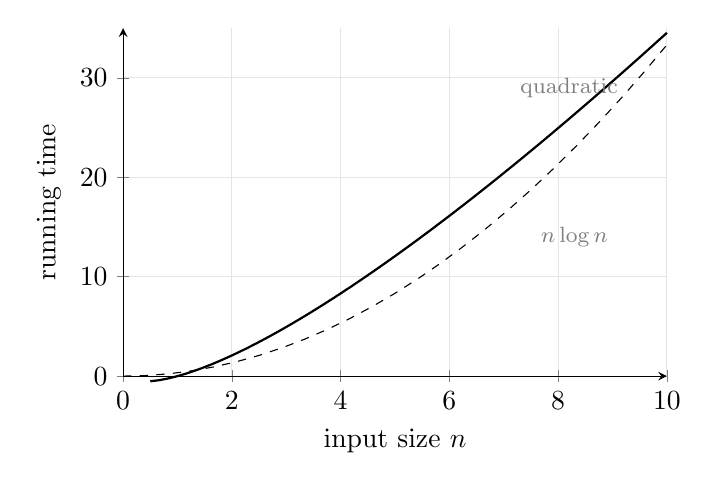
\begin{tikzpicture}
\begin{axis}[width=0.7\textwidth,height=6cm,xlabel={input size $n$},ylabel={running time},
  xmin=0,xmax=10,ymin=0,ymax=35,axis x line=bottom,axis y line=left,clip=false,grid=major,grid style={gray!20}]
  \addplot[domain=0.5:10,samples=60,thick]{x*ln(x)*1.5};
  \addplot[domain=0:10,dashed]{x^2/3};
  \node[font=\footnotesize,gray] at (axis cs:8.2,29) {quadratic};
  \node[font=\footnotesize,gray] at (axis cs:8.3,14) {$n\log n$};
\end{axis}
\end{tikzpicture}
\caption{Growth of two running-time curves (pgfplots).}
\end{figure}
\begin{figure}[H]
\centering
\begin{subfigure}[t]{0.45\textwidth}\centering
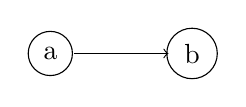
\begin{tikzpicture}\node[draw,circle]{a};\draw[->](0.3,0)--(1.5,0);\node[draw,circle] at (1.8,0){b};\end{tikzpicture}
\caption{First panel.}
\end{subfigure}\hfill
\begin{subfigure}[t]{0.45\textwidth}\centering
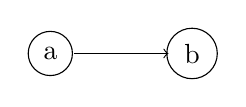
\begin{tikzpicture}\node[draw,circle]{a};\draw[->](0.3,0)--(1.5,0);\node[draw,circle] at (1.8,0){b};\end{tikzpicture}
\caption{Second panel.}
\end{subfigure}
\caption{Side-by-side subfigures.}
\end{figure}
